%!TEX root = ../thesis.tex
\chapter{Discussion \& Outlook}
\label{chap:discussion}


\section{Assessment of four and five dimensional approach}

During the reconstruction of an \ac{usct} image all the directional information of the transducers are lost. This is why Patrick Hucker \cite{PatrickHucker2014EvaluationRuckstreumodells} introduced a further dimension to his reconstructed images. The 4\textsuperscript{th} dimension can hold the directional information about the receiver directions or the emitter directions.

Why the 4\textsuperscript{th} dimension alone is not enough to characterise the reflection properties of different tissue types can be explained with a simple experiment:


\begin{figure}[H]
    \centering
    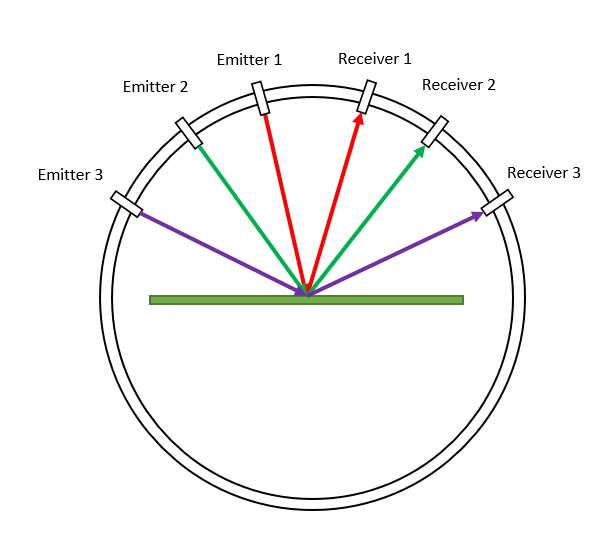
\includegraphics[width=0.56\textwidth]{Graphics/Diskussion/4D_not_enough.png}
    \caption{Experiment to prove that the 4\textsuperscript{th} dimensional approach is insufficient for analysing the reflection characteristics of a tissue. }
    \label{4D_sucks}
\end{figure}

In Figure \ref{4D_sucks} the aperture of the \ac{usct} device is shown. There are three emitters and three receivers. The green structure in the middle of the aperture is one big voxel which has an even surface and optimal specular reflection properties.

Because of the specularity of the surface, receiver 1 can only detect a pulse that originated from emitter 1. Analogously, receiver 2 can only detect the pulses from emitter 2 and receiver 3 can only receive a signal from emitter 3.

For the experiment three measurements are performed. For the first measurement only the first emitter is active and emits a pulse into the aperture. For the second measurement only the second and for the third measurement only the third emitter emits. During each of the three measurements all three receivers are active and measure the pressure. 

The recorded values are saved in a four dimensional image volume which is represented by the table in Figure \ref{table_2}: 

\begin{figure}[H]
    \centering
    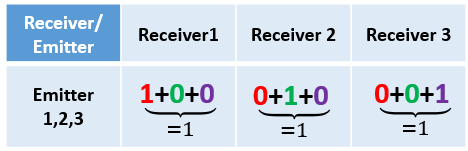
\includegraphics[width=0.56\textwidth]{Graphics/Diskussion/4D_not_enough_table_2.png}
    \caption{Measured values for four dimensional direction information.}
    \label{table_2}
\end{figure}

In the table there is a column for each receiver but only one row for the emitters. This is why emitters 1,2 and 3 are summarised in the one row.

During the first measurement receiver 1 is the only receiver that detected a signal. For this measurement receiver 1 gets a red one. The remaining receivers get a red zero. The same goes for the second measurement: Receiver 2 receives a signal (green one in table), receivers 1 and 3 do not (green zeros in table). Analogously, for the third measurement only the third receiver is assigned the purple one whereas the other receivers are assigned the purple zero.

\bigskip

After the last measurement, the sum of the recorded signals result in a one in each receiver column. The information about what emitter was the origin of which signal is lost. If we would try to make an assumption about the reflection characteristics of this particular voxel, we would probably assume that the voxel reflected uniformly in all directions and therefore has to have a diffuse reflection characteristic.

\bigskip

Alternatively, we could have saved the measurement results into a 5\textsuperscript{th} dimension. This is represented by the table in Figure \ref{table_1}:

\begin{figure}[H]
    \centering
    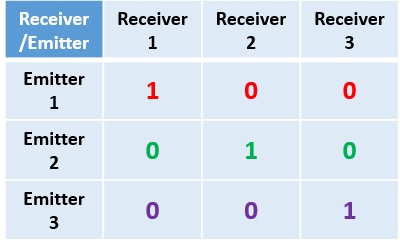
\includegraphics[width=0.56\textwidth]{Graphics/Diskussion/4D_not_enough_table.png}
    \caption{Measured values for five dimensional direction information.}
    \label{table_1}
\end{figure}

From this table we can reconstruct the emitter receiver configuration under which a signal was detected. Since only the leading diagonal of the table is occupied it becomes clear that the voxel has to have a specular reflection characteristic. 

\bigskip


For the classification of a reflection characteristic it is therefore inevitable to analyse both the emitter and the receiver directions of a voxel. These information can only be preserved if a 5\textsuperscript{th} dimension is introduced to the reconstructed image. During this thesis the previous implementation of Patrick Hucker was extended and the tools for the analysis of the reflection characteristics. For the five dimensional approach the information of original 3D image is distributed into all the sub images for each 4D-5D combination. To compensate the reduced contrast of the resulting sub images a suitable visualisation technique is presented (compare section \ref{chap:max_devi}). 

\newpage

\section{Resolution of the discretisation of direction}

The resolution of the discretisation has to be considered for the characterisation of the reflective properties of a tissue. This can be explained with an example in Figure \ref{fig:resolution_of_segmentation}. The example shows two bell curves that represent two different reflection characteristics of a tissue. The wider curve represents a mixed reflectivity with specular and diffuse parts. The narrow green curve represents a near specular scatterer. The goal is to distinguish between both curves. In the sub-figures there are three different levels of the resolution of the directional information shown.


\begin{figure}[H]
     \centering
     \begin{subfigure}[b]{0.32\textwidth}
         \centering
        \fbox{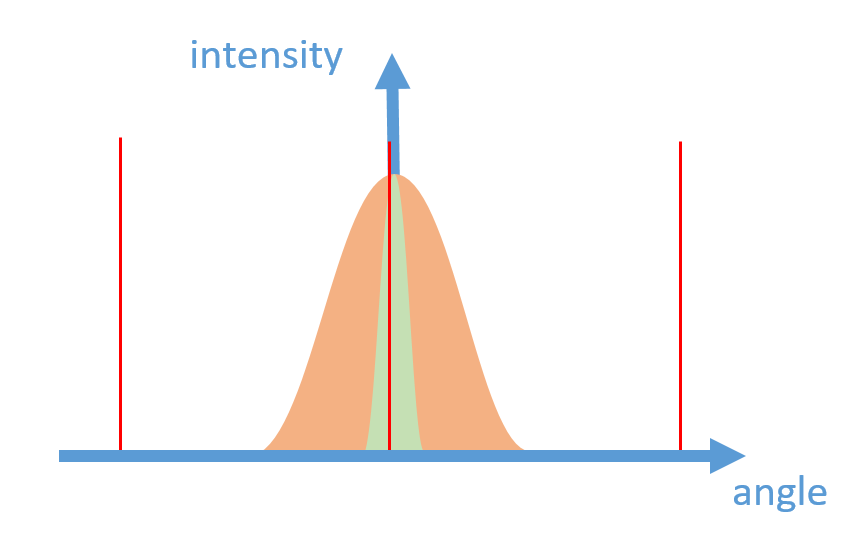
\includegraphics[width=0.8\linewidth]{Graphics/zuwenigaufloesung.png}}
         \caption{Insufficient resolution of the discretisation.}
         \label{fig:resolution_of_segmentation_wenig}
     \end{subfigure}
     \hfill
     \begin{subfigure}[b]{0.32\textwidth}
         \centering
         \fbox{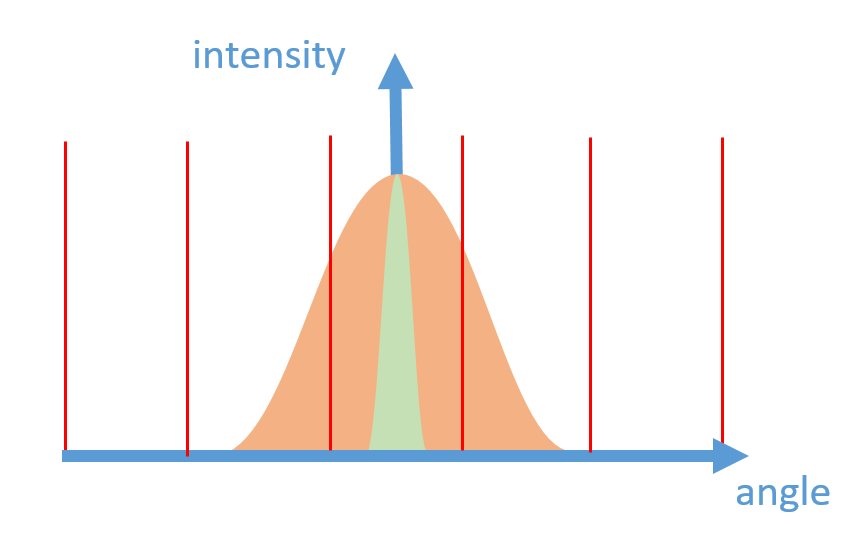
\includegraphics[width=0.8\textwidth]{Graphics/bessereaufloesung.png}}
         \caption{Better resolution of the discretisation.}
         \label{fig:resolution_of_segmentation_mittel}
     \end{subfigure}
     \hfill
     \begin{subfigure}[b]{0.32\textwidth}
         \centering
         \fbox{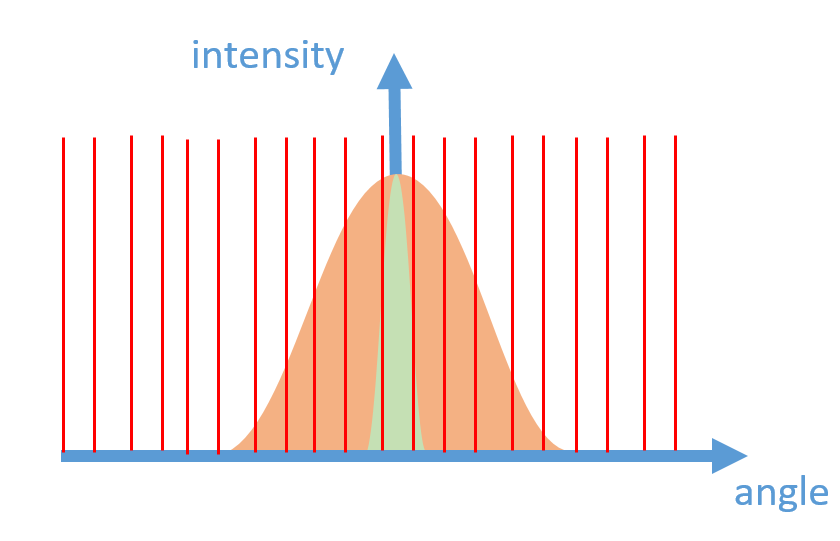
\includegraphics[width=0.8\textwidth]{Graphics/optimaleafloesung.png}}
         \caption{Optimal resolution of the discretisation.}
         \label{fig:resolution_of_segmentation_gut}
     \end{subfigure}
        \caption{Reflection characteristics of different surfaces and angle of incidence.}
        \label{fig:resolution_of_segmentation}
\end{figure}


In Figure \ref{fig:resolution_of_segmentation_wenig} the resolution of the directional information simply is not high enough to distinguish between both curves since they are both too narrow. The second solution shows a higher resolution of the discretisation of the directional information. The red lines are much closer to each other and the orange reflection characteristics can be analysed. To distinguish between the green and the orange curve the resolution is still insufficient. Figure \ref{fig:resolution_of_segmentation_gut} shows a near optimal solution for the problem. Both reflection characteristics could be distinguished. 

The introduction of the arbitrary directional segmentation allows to increase the resolution of the discretisation as desired and with that to increase the resolution of the segmentation. This is one of the main features that has been introduced during the thesis and allows the analysis of the different reflection characteristics. One of the challenges of the enhancement of the resolution of the segmentation is the increasing computation time. This issue was addressed by the introduction of a more efficient assignment method.






\section{Comparison of the assignment algorithms}
In section \ref{sec:index_ident} two approach for the assignment of the directional information were presented. The first method is the angle sorting approach which was introduced by Patrick Hucker.

It was extended from 4D to 5D during this thesis. The second method is the orthogonality threshold which was developed during this thesis. The main difference between both methods are the different decision criteria and the execution time. In section \ref{sec:index_ident} the different decision areas of both approaches were presented in detail. In the following the three decision criteria are compared:

\begin{figure}[H]
    \centering
    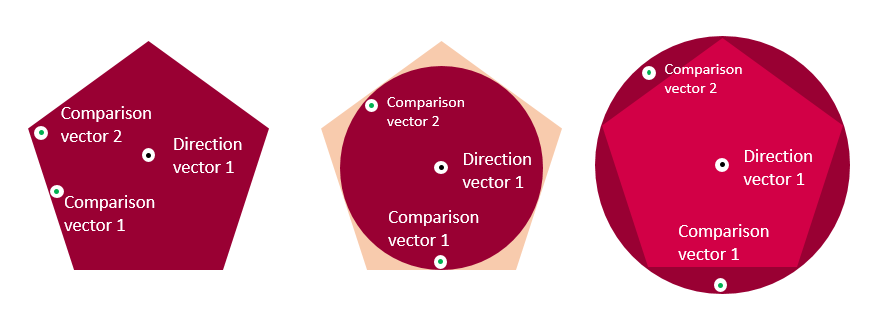
\includegraphics[width=0.76\textwidth]{Graphics/different_quality_assignment.png}
    \caption{Different decision areas of the angle sorting method (left) and the orthogonality threshold with enclosed decision area (middle) and with external decision area. }
    \label{angle_assignment_quality}
\end{figure}

For the \textbf{angle sorting} method there are fixed boundaries which correlate to the geometry of the configuration of directional vectors. For the 5D angle sorting method two different comparison vectors are assigned to the same directional vector. This can be seen in Figure \ref{angle_assignment_quality} on the left side. The comparison vector 1 is located at the boundary of the pentagon. Comparison vector 2 is located in one of the 'tips' of the pentagon where two boundaries meet. The distance from comparison vector 1 to the directional vector in the middle of the pentagon is smaller than the distance between comparison vector 2 and the directional vector. Still, both comparison vectors are assigned to the same directional vector. 
The decision area for the orthogonality threshold method is shown on the right side. The comparison vector 1 and 2 are both located on the boundary of the decision area. Both have the same distance to the directional vector 1 in the middle of the circle. 

Two comparison vectors that are located at the boundary of the same decision area can have a different angle to the comparison vector. For the angle sorting method both direction vectors may be assigned to the same directional vector. This leads to the conclusion that the angle sorting method has a varying quality of assignment. It can not be guaranteed that two comparison vectors that have the same angle to same directional vector are both assigned to the directional vector. 

\bigskip


The \textbf{orthogonality threshold} method treats all directional vectors equally and guarantees a constant quality of the assignment. If the threshold is chosen as the enclosed circle of the pentagon (compare Figure \ref{angle_assignment_quality} (middle)) some \acp{ascan} may be not regarded which results in a lower contrast of the image. On the other hand, this method leads to a distinct assignment.

The other possibility is to chose the decision areas to be overlapping. An example is given in Figure \ref{angle_assignment_quality} (right). For this case still a constant quality of the assignment can be assured and in addition to that all \acp{ascan} can be considered.

\bigskip

The other big difference between the two algorithms is their performance. While the angle sorting method iterates over every possible directional vector during the assignment process, the orthogonality threshold method needs only are previously calculated threshold for that one set of directional vectors and can compare the comparison vectors to this threshold. That increases the performance of the algorithm considerably. Both methods have to be executed multiple times during the reconstruction. To be precise for a full reconstruction there are $1.982x10^{16}$ calculations necessary where the assignment methods are involved. Therefore, this big difference in performance for more directional vectors makes the angle sorting approach to a bad choice. For small sets of directional vectors the impact may be not that big. With a rising number of directional vectors the threshold orthogonality method has its advantages in performance and the quality of the assignment process.  


Consequently, a trade-off has to be found between the advantages and disadvantages of the orthogonality method (uniqueness, contrast, vs. shorter computation time) and the angle search (potentially higher contrast vs. non-equal angular distribution of content and longer computation times). This thesis laid the groundwork which allows the analysis of the influence of the different decision criteria in the future with more data.





%\section{Advantages of looping implementation}

%-> Kein Meomory overflow

%\section{Alternative implementation of reconstruction}

%-> Directly in c++ code not as loop


\section{Interpretation of visualisation of the reflection characteristics}
\label{chap:max_devi}

For the comprehensible visualisation of the five dimensional data the deviation imaging and maximum imaging approach was presented. For each voxel in the measurement volume the directional data was interpreted and a three dimensional representation of the data was found. From the deviation and maximum images a first distinction between the specular and diffuse behaviour of a material was made possible. For the exact determination of different tissue types further evaluations are required. In particular the deviation approach lead to a suppression of the ellipsoidal artefacts in the image. These results might be suitable as input data for a machine learning algorithm which eventually could classify different tissues. Furthermore the relatively sharp representation of the surfaces could prove helpful for the segmentation of the tissue.


\section{Discussion of the implementation of the methods}

The multidimensional reconstruction was implemented in a way that two separate images are reconstructed for each directional vector. The biggest disadvantage of this method is the computation time of the reconstruction which increases linearly with the number of direction vectors. On the other hand, during the run time of the reconstruction algorithm of the old implementation, the assignment process needed to hold the whole image volume in the memory of the \acp{gpu}. This limit was overcome by calling the reconstruction multiple times and increasing the overall reconstruction time but also keeping the memory load of the \ac{gpu} constantly low. A next step would be to transfer the prototypically implemented MATLAB code into the CUDA kernel of the reconstruction. The implementation of the reconstruction for the five dimensional images was designed to be parallelisable and it can be partitioned arbitrarily.




\section{Conclusion \& Outlook}

The previous methods presented by Patrick Hucker \cite{PatrickHucker2014EvaluationRuckstreumodells} had inherent features that prevented the reconstruction of five dimensional volumes and with that made the successful classification of reflection characteristics improbable. The introduction of a 5\textsuperscript{th} dimension during this thesis brought us a big step closer to the classification of tissues by analysing the reflection characteristics. The inability to increase the resolution of the segmentation of the directional information arbitrarily was addressed during this thesis. A generalisation of the problem lead to new approach which allows to arbitrarily increase the resolution of the discretisation of the directional information. This new method lay the  groundwork for the detection of narrow reflection characteristics (e.g. specularity).

Moreover, the performance of the novel orthogonality threshold method was compared to the angle sorting method. The analysis concluded that the execution time per function call of the angle sorting method grew quadratically with the amount of directional vectors for the old method. This makes the old method unattractive for the assignment process with a high resolution of the discretisation. The execution time of the orthogonality method showed a linear behaviour with increasing numbers of direction vectors. This makes this method more suitable for high resolution applications. Non-overlapping decision areas were chosen for the current implementation of the orthogonality threshold to assure an unambiguous assignment to the directional vectors. The decision criteria could possibly be extended by weighting the assigned voxel values based on the orthogonality or distance to the directional vector. The influence of the different decision criteria on the resulting deviation and max images could be pursued in future.


The overall goal of this thesis was to provide insights into the reflection characteristics of different types of tissue and with these information increase the value of the reconstructed \ac{usct}-images. The distinguishing of tissue types with with near specular reflection properties from diffuse scatterers could be achieved with the introduction of the deviation imaging. This insight could prove helpful in future works for recognising different breast tissues and can possibly aid in the tumour detection.









